\chapter{Gestures Evaluation And Results}
The evaluation of the static approaches were done using RapidMiner[link to it] in an Intel celeron (2 GH) computer with 2GB DDR3.\bigskip

The algorithms defined in classification chapter (K-NN, Naive Bayes, SVM) were applied to our dataset, and the experiments were performed under the assumption of the k-fold method. The k-fold cross validation is used to determine how accurately a learning algorithm wil be able to predict data that it was not trained with[link here]. In the k-fold cross-validation, the dataset X is divided randomly into k equal sized parts. The learning algorithm is then trained k times, using k-1 parts as trainning set and the one as test set. A value of k=10 is used, giving a good rule of approximation.
\bigskip

The results obtained with the data-set are represented in the following table:\bigskip

\begin{center}
\begin{tabular}{ |c|c|c|c| }
 \hline
 Approach/Classifier & K-NN & SVM & Naive-Bayes \\
 \hline
 Approach 1 & 96.42 \%  & 88.74 \%  & 90 \%  \\
 \hline
 Approach 2 & 87.76 \%  & 78.57 \%  & 81 \%  \\
 \hline
 Approach 3 & 92.95 \%  & 85.79 \%  & 86.79 \% \\
 \hline
\end{tabular}
\end{center}


To analyze how classification errors are distributed among classes we computed for each trained algorithm it's coresponding confusing matrix has shown in the following figures.\bigskip

\begin{figure*}[h]
\begin{dBox}
\centering
 \mbox{
     \subfigure[]{
            \label{fig:apr1knn}
            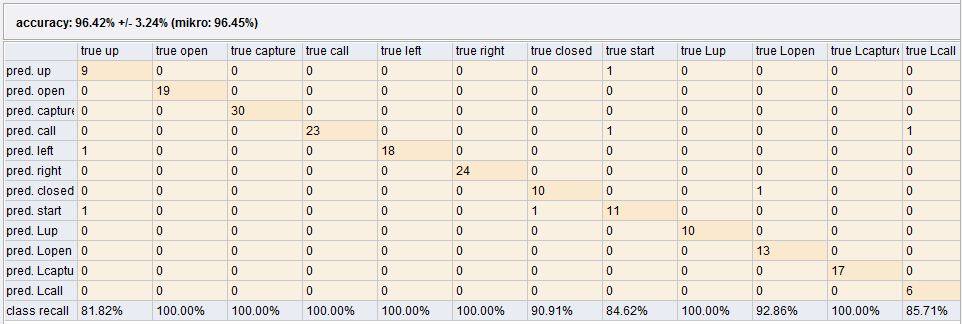
\includegraphics[width=.9\textwidth]{./Pictures/gesture/R_K-NN_B.jpg}
        }
  }
  \caption{Approach 1 K-NN\label{fig:apr1_knn} }   
\end{dBox}   
\end{figure*}

\begin{figure*}[h]
\begin{dBox}
\centering
 \mbox{
     \subfigure[]{
            \label{fig:apr2knn}
            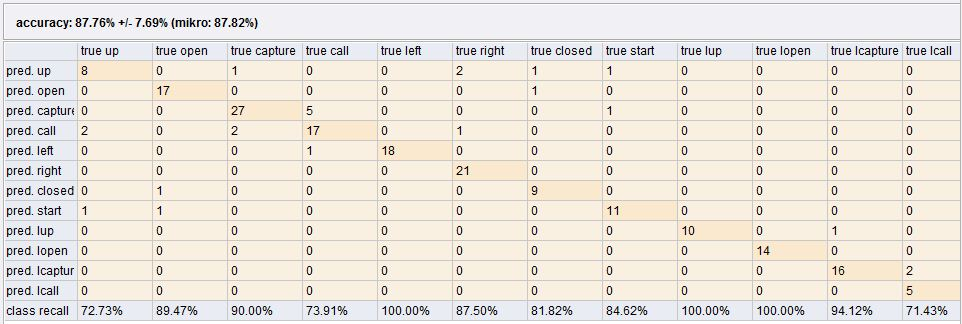
\includegraphics[width=.9\textwidth]{./Pictures/gesture/R_K-NN_F.jpg}
        }
  }
  \caption{Approach 2 K-NN\label{fig:apr2_knn} }
  
\end{dBox}   
\end{figure*}

\begin{figure*}[h]
\begin{dBox}
\centering
 \mbox{
     \subfigure[]{
            \label{fig:apr3knn}
            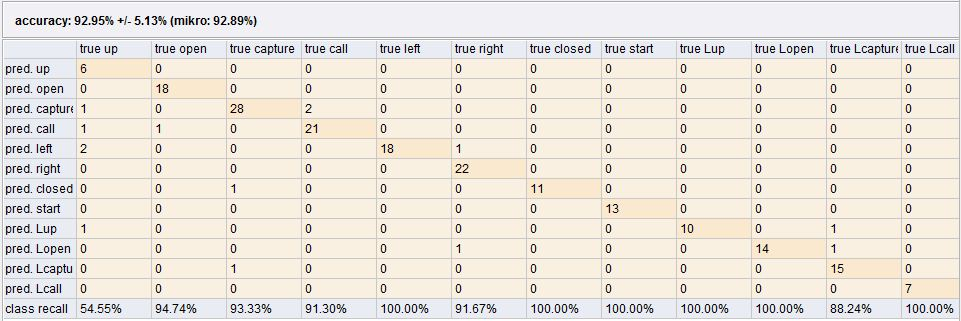
\includegraphics[width=.9\textwidth]{./Pictures/gesture/R_K-NN_SIFT.jpg}
        }
  }
  \caption{Approach 3 K-NN\label{fig:apr3_knn} } 
\end{dBox}   
\end{figure*}
% end of k-nn figures

\begin{figure*}[h]
\begin{dBox}
\centering
 \mbox{
     \subfigure[]{
            \label{fig:apr1svm}
            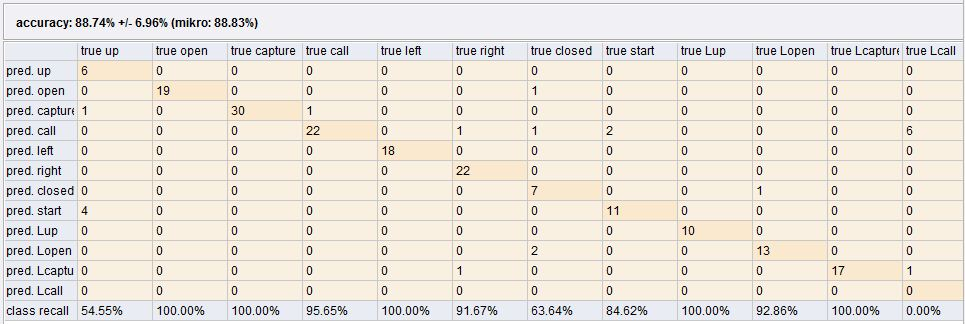
\includegraphics[width=.9\textwidth]{./Pictures/gesture/R_SVM_Binary.jpg}
        }
  }
  \caption{Approach 1 SVM\label{fig:apr1_svm} }   
\end{dBox}   
\end{figure*}

\begin{figure*}[h]
\begin{dBox}
\centering
 \mbox{
     \subfigure[]{
            \label{fig:apr2svm}
            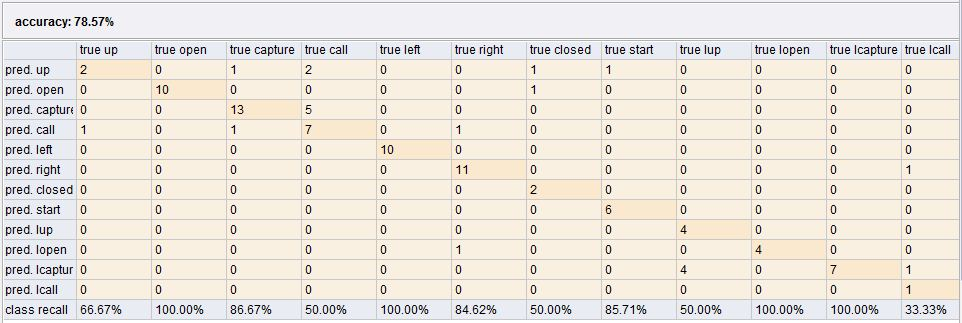
\includegraphics[width=.9\textwidth]{./Pictures/gesture/R_SVM_Feature.jpg}
        }
  }
  \caption{Approach 2 SVM\label{fig:apr2_svm} }
  
\end{dBox}   
\end{figure*}
\begin{figure*}[h]
\begin{dBox}
\centering
 \mbox{
     \subfigure[]{
            \label{fig:apr3svm}
            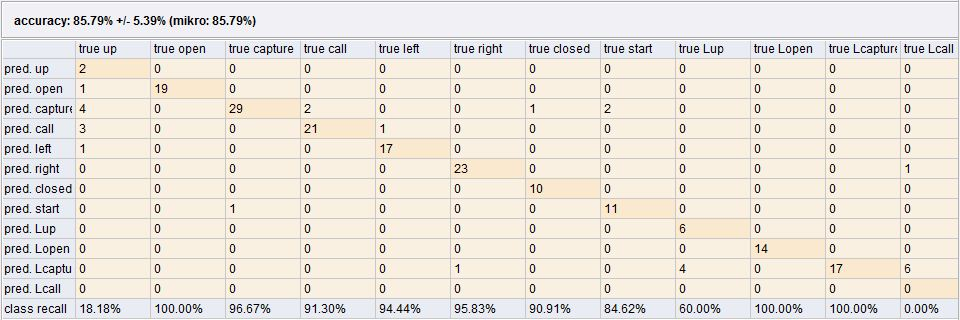
\includegraphics[width=.9\textwidth]{./Pictures/gesture/R_SVM_SIFT.jpg}
        }
  }
  \caption{Approach 3 SVM\label{fig:apr3_svm} } 
\end{dBox}   
\end{figure*}
% end of svm
% bayes lsaaaa
